% 以下の3行は変更しないこと.
\documentclass[T]{compsoft}
\taikai{2021}
\pagestyle {empty}

\usepackage [dvipdfmx] {graphicx}
\usepackage [dvipdfmx] {color}

% ここに,使用するパッケージを列挙する.
\usepackage{amsthm,amsmath,amssymb}
\usepackage{url}
\usepackage{enumerate,mathdots} % 箇条書き・左下向きの3点リーダー
\usepackage{tikz,here} % 図・コード
\usetikzlibrary{intersections,calc,arrows.meta,positioning}

% ユーザが定義したマクロなどはここに置く.
% ただし学会誌のスタイルの再定義は原則として避けること.
\usepackage{mymacro}
\usepackage{mystyle}

% コマンド一覧
%\def\colorF{\textit{color}}
\def\topcolor{\textit{topcol}}
\def\Color{\textit{Color}}
\def\mix{\textit{mix}}
\def\red{\textit{red}}
\def\blu{\textit{blu}}
\def\yel{\textit{yel}}
\def\mix{\textit{mix}}
\def\colorYB{\textit{colorYB}}
\def\colorBYB{\textit{colorBYB}}
\def\colorYBBY{\textit{colorYBBY}}
\def\cposF{\textit{cposF}}
\def\cposYB{\textit{cposYB}}
\def\cposBYB{\textit{cposBYB}}
\def\cposYBBY{\textit{cposYBBY}}
\def\lift{\textit{liftpaint}}
\def\cpos{\textit{cpos}}
\def\Cpos{\textit{Cpos}}
\def\WCTF{\textit{Triangle}}
\def\TF{\textit{TriangleF}}
\def\WCT{\textit{WellColoredTriangle}}
\def\WCTF{\textit{WellColoredTriangleF}}
\def\mixCut{\textit{mixCut}}
\def\AllRed{\textit{AllRed}}
\def\falseColor{\textit{falseColor}}
\def\Cexists{\textit{C\_exists}}
\def\Cuniq{\textit{C\_uniq}}
\def\Cmix{\textit{C\_mix}}
\def\Cpaint{\textit{C\_paint}}
\def\Fmix{\textit{Fmix}}
\def\EvenA{\textit{EvenA}}
\def\EvenB{\textit{EvenB}}
\def\Even{\textit{Even}}
\def\ShortOddA{\textit{ShortOddA}}
\def\ShortOddB{\textit{ShortOddB}}
\def\ShortOddC{\textit{ShortOddC}}
\def\ShortOdd{\textit{ShortOdd}}
\def\LongOddA{\textit{LongOddA}}
\def\LongOddB{\textit{LongOddB}}
\def\LongOddC{\textit{LongOddC}}
\def\LongOdd{\textit{LongOdd}}

\begin{document}

% 論文のタイトル
\title{
  Coq による三角形三色問題の証明
}

\author{橋本 翔太 木村 大輔
  %
  % ここにタイトル英訳 (英文の場合は和訳) を書く.
  \ejtitle{
    A formal proof for the three-colored triangle problem on Coq
  }
  %
  % 所属 (和文および英文) を書く.複数著者の所属はまとめてよい.
  \shozoku{Shota Hashimoto}{東邦大学大学院理学研究科}%
  {Toho University}  
  \shozoku{Daisuke Kimura}{東邦大学大学院理学研究科}%
  {Toho University}
  %
  \shutten
  \uketsuke{2099}{99}{99} % dummy
}


\Jabstract{
  Coq とは数学の証明作成を支援するプログラミング言語である.Coq と人間は対話的なやりとりをしながら証明作成をおこなうことで誤りを排除した信頼できる証明を得られる. 三角形三色問題とは $n$ 段の逆三角形に配置された六角形のマスに対して,隣り合う2マスとそれらに接する下の段のマスの色が3色とも同じか3色とも異なるように3色で塗り分けたとき,逆三角形の端点の3マスの色も3色とも同じか3色とも異なるような段数の一般項を求める問題である.この問題は雑誌「数学セミナー」の「エレガントな解答もとむ」欄に出題されており,一般項は $3^k$ 段の形で表せることが示されている.本研究では,数学セミナーでの証明をCoqで形式化して証明を完成させた. Coq に実装する際には,幾何的な直観に頼った側面のある元の議論を論理に基づいた形式的な証明に直すことができた.
}

\maketitle \thispagestyle {empty}

% 導入
\section{はじめに}
% Coq + ssreflect の説明
Coq~\cite{Coq} とは数学の定理や補題,主張の正しさを保証するためのソフトウェアの$1$つである.
証明の作成中の各場面で示すべき主張(サブゴール)に対して人間がサブゴールを示すための次の一手を指示するとCoqは次のサブゴールを提示し,人間の次の一手を待つ.
このような対話的なやりとりによりCoqは証明の完成の手助けをする.こういったソフトウェアを定理証明支援系と呼ぶ.
証明の規模が大きくなると,複雑な場合分けの漏れがあったり計算ミスなど機械的操作のミスにより人間は誤った証明をしてしまうことがある.
Coq の支援を受けることで,このような誤りが排除された信頼できる証明を得ることができる.
また,Coq はプログラミング言語でもあるため,作成した証明の複製が容易である.
Coq を用いて作成した証明ファイルを公開することで他の人がライブラリとして利用することができる.
既に示された定理は保証済みのものとして,多くの人が各々の目的達成のために利用することができる.
このように,公開された証明1つ1つがたとえ小さな証明であっても組み合わせることで規模の大きな証明の定理を示しやすくなる.

本研究では,Coq + SSReflect を用いて三角形三色問題の証明の形式化を完成させた.
SSReflect~\cite{SSReflect,CoqBook} は「証明によるリーズニングよりも計算を積極的に用いた方が証明は簡略化される」(ポワンカレ原理)の
ポリシーに基づいて設計された Coq の拡張ライブラリである.

三角形三色問題~\cite{Nishiyama1,Nishiyama2,Nishiyama3}とは,次のような問題である:$n$段の逆三角形に配置された正六角形のすべてのマスを異なる3色を用いて色分けをする.ただし,隣り合う2マスとそれらに接する下の段のマスの色は,どれも同じかどれも異なるように塗り分ける.このとき,逆三角形の段数が 3, 9, 27 段の場合 \footnote{本稿では0段目, 1段目, 2段目,$\ldots$と数える.「$n$段の逆三角形」と書いた場合,一辺のマスの個数は$n+1$個である.} は,規則に従ったどのような色の塗り方をしても逆三角形の端点の3マスの色はどれも同じかどれも異なるが,一般にはこのような性質は成り立たない.このような性質を満たす段数の一般項は何か?という問題である.この問題の解決方法は大きく分けて3つの方法が知られている.\cite{Nishiyama1}
\begin{enumerate}
\item \label{ans_1}
  パスカルの三角形の値をmod $3$としたものをマスの色と対応させて使い,代数学での $Lucas$ の定理と関係のある命題を示すことで解決する方法.
\item \label{ans_2}
  逆三角形のマスの塗り方が$n$個の独立パターンに分解できること利用して,重ね合わせの原理を用いることで解決する方法.
\item \label{ans_3}
  比較的少ない段数で成立する段数を調べて段数の規則性(数列)を見つけ出し,この数列から予測できる段数の一般項を推測する方法.
\end{enumerate}
\ref{ans_3}の方法において一般項が$3^k$段であると推測されており,推測された一般項の段数でないならば逆三角形の塗り方の規則に従わない反例が存在することも知られている.

% やったこと
本研究では\ref{ans_3}.の方法で推測して得られた一般項が必要十分条件になっていることを Coq+SSReflect を用いて証明した.
Coq に実装するにあたって,三角形三色問題は幾何的な側面を多くもつ問題であるためこのままでは Coq にコードとして実装することができない.
そこで,三角形のマスの状況を表現する論理式を用意し,色塗り規則を公理化することで三角形三色問題の状況を形式化した.
また,十分条件の証明の方法としては一般項に現れる自然数$k$に関する数学的帰納法を用いて証明した.
一方で,必要条件は対偶法と$n$について場合分けをすることで証明した.

% もくじ
本論文は
第$2$章では三角形三色問題の証明の概要について述べる.
第$3$章では三角形三色問題の証明をCoqに実装するために必要な準備について述べる.
第$4$章では実際にCoqに実装した三角形三色問題の証明について述べる.

% 三角形三色問題の概要(数学)
% 調和彩色三角形 (well-colored triangle)
% 彩色三角形が調和している
% 彩色三角形が調和性をみたす
\section{三角形三色問題の概要}
三角形三色問題について述べる前に調和性と調和彩色三角形の定義について先に述べる.
以下,$3$色のどれかの色が塗られた同じ大きさの正六角形のマスが平面上に逆三角形の形に敷き詰められている状況を考える (図~\ref{fig:nine_steps}参照)
\footnote{
  塗られる色は青,赤,黄を想定しているが,図の中では紙面の都合を考慮してそれぞれ黒,灰色,白に変換している.
}.

\begin{dfn}[調和性] \label{dfn:wc}\rm
  (隣接しているとは限らない) $3$つのマスに塗られている色がすべて同じか相異なるとき,
  この$3$マスは{\em 調和性}を満たすという.
\end{dfn}

\begin{exm}
  図$\ref{wellcoloed}$のような$3$マスの組は調和性を満たしているが,
  図$\ref{notwellcoloed}$のような$3$マスの組は調和性を満たしていない.
  \begin{figure}[h]
    \centering
    % wellcolored
\begin{tikzpicture}[scale=0.25]
  % 左図
  \begin{scope}[xshift={-150}]
    \myHexB{-1}{1}
    \myHexY{1}{1}
    \myHexR{0}{0}
  \end{scope}
  % 右図  
  \begin{scope}[xshift={150}]
    \myHexY{-1}{1}
    \myHexY{1}{1}
    \myHexY{0}{0}
  \end{scope}
\end{tikzpicture}

    \caption{調和性を満たす$3$色の組}
    \label{wellcoloed}
  \end{figure}
  \begin{figure}[h]
    \centering
    % wellcolored
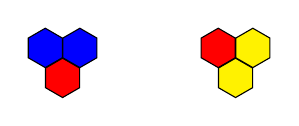
\begin{tikzpicture}[scale=0.25]
  %1段目
  \filldraw[fill=red,xshift={-25*5},yshift={25*sqrt(3)*3}] (0,0)--++(30:1)--++(90:1)--++(150:1)--++(210:1)--++(270:1)--cycle;
  \filldraw[fill=yellow,xshift={25*5},yshift={25*sqrt(3)*3}] (0,0)--++(30:1)--++(90:1)--++(150:1)--++(210:1)--++(270:1)--cycle;
  %0段目
  \filldraw[fill=blue,xshift={-25*4},yshift={25*sqrt(3)*4}] (0,0)--++(30:1)--++(90:1)--++(150:1)--++(210:1)--++(270:1)--cycle;
  \filldraw[fill=blue,xshift={-25*6},yshift={25*sqrt(3)*4}] (0,0)--++(30:1)--++(90:1)--++(150:1)--++(210:1)--++(270:1)--cycle;
  \filldraw[fill=yellow,xshift={25*6},yshift={25*sqrt(3)*4}] (0,0)--++(30:1)--++(90:1)--++(150:1)--++(210:1)--++(270:1)--cycle;
  \filldraw[fill=red,xshift={25*4},yshift={25*sqrt(3)*4}] (0,0)--++(30:1)--++(90:1)--++(150:1)--++(210:1)--++(270:1)--cycle;
\end{tikzpicture}

    \caption{調和性を満たさない$3$色の組}
    \label{notwellcoloed}
  \end{figure}
\end{exm}

\begin{dfn}[彩色三角形] \label{dfn:three_tri}\rm
  隣接した全ての$3$マスが調和性を満たすように色が塗られた逆三角形を
  {\em 彩色三角形}という.
\end{dfn}

\begin{dfn}[調和彩色三角形] \label{dfn:wc_tri}\rm
  $3$つの端点のマスに塗られている色が調和性を満たしている彩色三角形を{\em 調和彩色三角形} (well-colored triangle) という.
\end{dfn}

次に三角形三色問題について述べる.
  $n(>0)$段の彩色三角形がある.
  図\ref{fig:nine_steps}は$n=9$のときの彩色三角形である.
  このとき,最下段のマスの色は赤であり,最上段の両端のマスは黄,青であるから
  最上段の両端のマスの色と最下段のマスの色について調和性を満たしている (つまり,調和彩色三角形である) ことが分かる.

\begin{figure}[h]
    \centering
    % 9steps
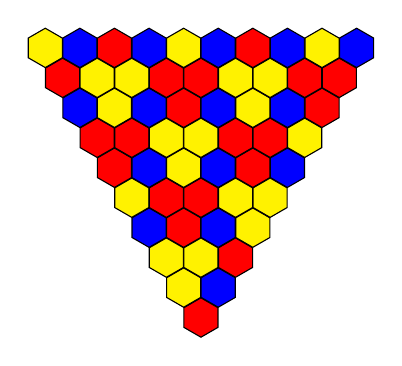
\begin{tikzpicture}[scale=0.25]
  %9段目
  \filldraw[fill=red] (0,0)--++(30:1)--++(90:1)--++(150:1)--++(210:1)--++(270:1)--cycle;
  %8段目
  \filldraw[fill=yellow,xshift={-25},yshift={25*sqrt(3)}] (0,0)--++(30:1)--++(90:1)--++(150:1)--++(210:1)--++(270:1)--cycle;
  \filldraw[fill=blue,xshift={25},yshift={25*sqrt(3)}] (0,0)--++(30:1)--++(90:1)--++(150:1)--++(210:1)--++(270:1)--cycle;
  %7段目
  \filldraw[fill=yellow,xshift={-25*2},yshift={25*sqrt(3)*2}] (0,0)--++(30:1)--++(90:1)--++(150:1)--++(210:1)--++(270:1)--cycle;
  \filldraw[fill=yellow,yshift={25*sqrt(3)*2}] (0,0)--++(30:1)--++(90:1)--++(150:1)--++(210:1)--++(270:1)--cycle;
  \filldraw[fill=red,xshift={25*2},yshift={25*sqrt(3)*2}] (0,0)--++(30:1)--++(90:1)--++(150:1)--++(210:1)--++(270:1)--cycle;
  %6段目
  \filldraw[fill=blue,xshift={-25*3},yshift={25*sqrt(3)*3}] (0,0)--++(30:1)--++(90:1)--++(150:1)--++(210:1)--++(270:1)--cycle;
  \filldraw[fill=red,xshift={-25},yshift={25*sqrt(3)*3}] (0,0)--++(30:1)--++(90:1)--++(150:1)--++(210:1)--++(270:1)--cycle;
  \filldraw[fill=blue,xshift={25},yshift={25*sqrt(3)*3}] (0,0)--++(30:1)--++(90:1)--++(150:1)--++(210:1)--++(270:1)--cycle;
  \filldraw[fill=yellow,xshift={25*3},yshift={25*sqrt(3)*3}] (0,0)--++(30:1)--++(90:1)--++(150:1)--++(210:1)--++(270:1)--cycle;
  %5段目
  \filldraw[fill=yellow,xshift={-25*4},yshift={25*sqrt(3)*4}] (0,0)--++(30:1)--++(90:1)--++(150:1)--++(210:1)--++(270:1)--cycle;
  \filldraw[fill=red,xshift={-25*2},yshift={25*sqrt(3)*4}] (0,0)--++(30:1)--++(90:1)--++(150:1)--++(210:1)--++(270:1)--cycle;
  \filldraw[fill=red,yshift={25*sqrt(3)*4}] (0,0)--++(30:1)--++(90:1)--++(150:1)--++(210:1)--++(270:1)--cycle;
  \filldraw[fill=yellow,xshift={25*2},yshift={25*sqrt(3)*4}] (0,0)--++(30:1)--++(90:1)--++(150:1)--++(210:1)--++(270:1)--cycle;
  \filldraw[fill=yellow,xshift={25*4},yshift={25*sqrt(3)*4}] (0,0)--++(30:1)--++(90:1)--++(150:1)--++(210:1)--++(270:1)--cycle;
  %4段目
  \filldraw[fill=red,xshift={-25*5},yshift={25*sqrt(3)*5}] (0,0)--++(30:1)--++(90:1)--++(150:1)--++(210:1)--++(270:1)--cycle;
  \filldraw[fill=blue,xshift={-25*3},yshift={25*sqrt(3)*5}] (0,0)--++(30:1)--++(90:1)--++(150:1)--++(210:1)--++(270:1)--cycle;
  \filldraw[fill=yellow,xshift={-25*1},yshift={25*sqrt(3)*5}] (0,0)--++(30:1)--++(90:1)--++(150:1)--++(210:1)--++(270:1)--cycle;
  \filldraw[fill=blue,xshift={25*1},yshift={25*sqrt(3)*5}] (0,0)--++(30:1)--++(90:1)--++(150:1)--++(210:1)--++(270:1)--cycle;
  \filldraw[fill=red,xshift={25*3},yshift={25*sqrt(3)*5}] (0,0)--++(30:1)--++(90:1)--++(150:1)--++(210:1)--++(270:1)--cycle;
  \filldraw[fill=blue,xshift={25*5},yshift={25*sqrt(3)*5}] (0,0)--++(30:1)--++(90:1)--++(150:1)--++(210:1)--++(270:1)--cycle;
  %3段目
  \filldraw[fill=red,xshift={-25*6},yshift={25*sqrt(3)*6}] (0,0)--++(30:1)--++(90:1)--++(150:1)--++(210:1)--++(270:1)--cycle;
  \filldraw[fill=red,xshift={-25*4},yshift={25*sqrt(3)*6}] (0,0)--++(30:1)--++(90:1)--++(150:1)--++(210:1)--++(270:1)--cycle;
  \filldraw[fill=yellow,xshift={-25*2},yshift={25*sqrt(3)*6}] (0,0)--++(30:1)--++(90:1)--++(150:1)--++(210:1)--++(270:1)--cycle;
  \filldraw[fill=yellow,yshift={25*sqrt(3)*6}] (0,0)--++(30:1)--++(90:1)--++(150:1)--++(210:1)--++(270:1)--cycle;
  \filldraw[fill=red,xshift={25*2},yshift={25*sqrt(3)*6}] (0,0)--++(30:1)--++(90:1)--++(150:1)--++(210:1)--++(270:1)--cycle;
  \filldraw[fill=red,xshift={25*4},yshift={25*sqrt(3)*6}] (0,0)--++(30:1)--++(90:1)--++(150:1)--++(210:1)--++(270:1)--cycle;
  \filldraw[fill=yellow,xshift={25*6},yshift={25*sqrt(3)*6}] (0,0)--++(30:1)--++(90:1)--++(150:1)--++(210:1)--++(270:1)--cycle;
  %2段目
  \filldraw[fill=blue,xshift={-25*7},yshift={25*sqrt(3)*7}] (0,0)--++(30:1)--++(90:1)--++(150:1)--++(210:1)--++(270:1)--cycle;
  \filldraw[fill=yellow,xshift={-25*5},yshift={25*sqrt(3)*7}] (0,0)--++(30:1)--++(90:1)--++(150:1)--++(210:1)--++(270:1)--cycle;
  \filldraw[fill=blue,xshift={-25*3},yshift={25*sqrt(3)*7}] (0,0)--++(30:1)--++(90:1)--++(150:1)--++(210:1)--++(270:1)--cycle;
  \filldraw[fill=red,xshift={-25*1},yshift={25*sqrt(3)*7}] (0,0)--++(30:1)--++(90:1)--++(150:1)--++(210:1)--++(270:1)--cycle;
  \filldraw[fill=blue,xshift={25*1},yshift={25*sqrt(3)*7}] (0,0)--++(30:1)--++(90:1)--++(150:1)--++(210:1)--++(270:1)--cycle;
  \filldraw[fill=yellow,xshift={25*3},yshift={25*sqrt(3)*7}] (0,0)--++(30:1)--++(90:1)--++(150:1)--++(210:1)--++(270:1)--cycle;
  \filldraw[fill=blue,xshift={25*5},yshift={25*sqrt(3)*7}] (0,0)--++(30:1)--++(90:1)--++(150:1)--++(210:1)--++(270:1)--cycle;
  \filldraw[fill=red,xshift={25*7},yshift={25*sqrt(3)*7}] (0,0)--++(30:1)--++(90:1)--++(150:1)--++(210:1)--++(270:1)--cycle;
  %1段目
  \filldraw[fill=red,xshift={-25*8},yshift={25*sqrt(3)*8}] (0,0)--++(30:1)--++(90:1)--++(150:1)--++(210:1)--++(270:1)--cycle;
  \filldraw[fill=yellow,xshift={-25*6},yshift={25*sqrt(3)*8}] (0,0)--++(30:1)--++(90:1)--++(150:1)--++(210:1)--++(270:1)--cycle;
  \filldraw[fill=yellow,xshift={-25*4},yshift={25*sqrt(3)*8}] (0,0)--++(30:1)--++(90:1)--++(150:1)--++(210:1)--++(270:1)--cycle;
  \filldraw[fill=red,xshift={-25*2},yshift={25*sqrt(3)*8}] (0,0)--++(30:1)--++(90:1)--++(150:1)--++(210:1)--++(270:1)--cycle;
  \filldraw[fill=red,yshift={25*sqrt(3)*8}] (0,0)--++(30:1)--++(90:1)--++(150:1)--++(210:1)--++(270:1)--cycle;
  \filldraw[fill=yellow,xshift={25*2},yshift={25*sqrt(3)*8}] (0,0)--++(30:1)--++(90:1)--++(150:1)--++(210:1)--++(270:1)--cycle;
  \filldraw[fill=yellow,xshift={25*4},yshift={25*sqrt(3)*8}] (0,0)--++(30:1)--++(90:1)--++(150:1)--++(210:1)--++(270:1)--cycle;
  \filldraw[fill=red,xshift={25*6},yshift={25*sqrt(3)*8}] (0,0)--++(30:1)--++(90:1)--++(150:1)--++(210:1)--++(270:1)--cycle;
  \filldraw[fill=red,xshift={25*8},yshift={25*sqrt(3)*8}] (0,0)--++(30:1)--++(90:1)--++(150:1)--++(210:1)--++(270:1)--cycle;
  %0段目
  \filldraw[fill=yellow,xshift={-25*9},yshift={25*sqrt(3)*9}] (0,0)--++(30:1)--++(90:1)--++(150:1)--++(210:1)--++(270:1)--cycle;
  \filldraw[fill=blue,xshift={-25*7},yshift={25*sqrt(3)*9}] (0,0)--++(30:1)--++(90:1)--++(150:1)--++(210:1)--++(270:1)--cycle;
  \filldraw[fill=red,xshift={-25*5},yshift={25*sqrt(3)*9}] (0,0)--++(30:1)--++(90:1)--++(150:1)--++(210:1)--++(270:1)--cycle;
  \filldraw[fill=blue,xshift={-25*3},yshift={25*sqrt(3)*9}] (0,0)--++(30:1)--++(90:1)--++(150:1)--++(210:1)--++(270:1)--cycle;
  \filldraw[fill=yellow,xshift={-25*1},yshift={25*sqrt(3)*9}] (0,0)--++(30:1)--++(90:1)--++(150:1)--++(210:1)--++(270:1)--cycle;
  \filldraw[fill=blue,xshift={25*1},yshift={25*sqrt(3)*9}] (0,0)--++(30:1)--++(90:1)--++(150:1)--++(210:1)--++(270:1)--cycle;
  \filldraw[fill=red,xshift={25*3},yshift={25*sqrt(3)*9}] (0,0)--++(30:1)--++(90:1)--++(150:1)--++(210:1)--++(270:1)--cycle;
  \filldraw[fill=blue,xshift={25*5},yshift={25*sqrt(3)*9}] (0,0)--++(30:1)--++(90:1)--++(150:1)--++(210:1)--++(270:1)--cycle;
  \filldraw[fill=yellow,xshift={25*7},yshift={25*sqrt(3)*9}] (0,0)--++(30:1)--++(90:1)--++(150:1)--++(210:1)--++(270:1)--cycle;
  \filldraw[fill=blue,xshift={25*9},yshift={25*sqrt(3)*9}] (0,0)--++(30:1)--++(90:1)--++(150:1)--++(210:1)--++(270:1)--cycle;
\end{tikzpicture}

    \caption{彩色三角形($n=9$のとき)}
    \label{fig:nine_steps}
\end{figure}

$n=9$の場合は最上段の塗り方が図\ref{fig:nine_steps}の塗り方でなくとも逆三角形の$3$つの頂点のマスは調和性を満たすことが観察できる.
このことから次のような仮説が考えられる.
\begin{itemize}
  \item[(仮説)]
  最上段をどのように塗っても最上段の両端のマスの色と最下段のマスの色は調和性を満たす.
\end{itemize}

数学セミナー誌で出題された三角形三色問題は次の$2$つの問題のことである~\cite{Nishiyama2}.
\begin{enumerate}
\item \label{que:1}
  $n=9$のとき仮説が成立することを証明せよ.
\item \label{que:2}
  $n=9$以外に仮説が成立する段数が存在するか調べ,存在するならば$n$の一般式を求めよ.
\end{enumerate}

この問題については既に解答が得られており,
一般に$n=3^k$段の逆三角形において仮説が成立することを示す次の定理\ref{thm:tri_iff}が示されている.

\begin{thm} \label{thm:tri_iff}
  $n(>0)$段の逆三角形に配置されたマス対して,
  最上段のマスを$3$色で任意に塗ったとき
  \[
  (\exists k\in\N.n=3^k) \Leftrightarrow \text{$n$段の逆三角形は常に調和彩色三角形}.
  \]
\end{thm}

本節ではこの定理の証明を Coq で実装するにあたり,証明の概要について述べる.

% 2.1 n=3^k => 調和三角形
\subsection{十分条件}
定理\ref{thm:tri_iff}を証明するにあたって,十分条件と必要条件に分けて話を進める.
ここでは定理\ref{thm:tri_iff}の十分条件である補題\ref{lem:tri_suf}の証明の概要について述べる.
\begin{lem}[十分条件] \label{lem:tri_suf}
  $n$段の逆三角形に配置されたマス対して,
  \[
  (\exists k\in\N.n=3^k) \Imp \text{$n$段の逆三角形は常に調和彩色三角形}.
  \]
\end{lem}
補題\ref{lem:tri_suf}を証明するためには論理同値である次の命題を証明すればよい.
\[
\forall k\in\N.(n=3^k \Imp \text{$n$段の逆三角形は常に調和彩色三角形}).
\]
これは$k$に関する数学的帰納法を用いて証明する.
\begin{itemize}
\item
  $k=0$のときは$n=1$となり明らかに成立する.
\item
  $k$ のとき成立すると仮定する.
  すなわち,$3^{k}$段の逆三角形ならば常に調和彩色三角形であると仮定する.
  
  ここからは図\ref{fig:ind_steps}を用いて証明を進める.
  以下,左から$x$番目,上から$y$段目のマスを$\Masu^x_y$と書くことにし,
  このマスに塗られている色を$c^x_y$とする.
\begin{figure}[h]
    \centering
    % 3^{k+1} 段の三角形
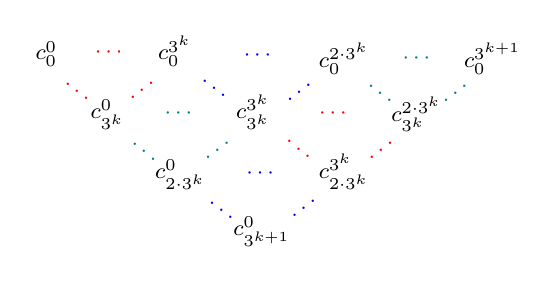
\begin{tikzpicture}
  {\footnotesize{
      % 3^(k+1)段目
      \node (a0) {$c^{0}_{3^{k+1}}$};
      % 2*3^k段目
      \node[above left=0.2cm of a0] (b0) {$c^{0}_{2\cdot3^{k}}$};
      \node[above right=0.2cm of a0] (b1) {$c^{3^{k}}_{2\cdot3^{k}}$};
      % 3^k段目
      \node[above left=0.25cm of b0] (c0) {$c^{0}_{3^{k}}$};
      \node[above right=0.25cm of b0] (c1) {$c^{3^{k}}_{3^{k}}$};
      \node[above right=0.1cm of b1] (c2) {$c^{2\cdot3^{k}}_{3^{k}}$};
      % 0段目
      \node[above left=0.3cm of c0] (d0) {$c^{0}_{0}$};
      \node[above right=0.3cm of c0] (d1) {$c^{3^{k}}_{0}$};
      \node[above left=0.1cm of c2] (d2) {$c^{2\cdot3^{k}}_{0}$};
      \node[above right=0.1cm of c2] (d3) {$c^{3^{k+1}}_{0}$};
      % 点線 [3^(k+1)段 〜 2*3^k 段]
      \node[blue] at ($(a0)!.5!(b0)$) {$\ddots$};
      \node[blue] at ($(b0)!.5!(b1)$) {$\cdots$};
      \node[blue] at ($(a0)!.5!(b1)$) {$\iddots$};
      % 点線 [2*3^k 段 〜 3^k 段]
      \node[teal] at ($(b0)!.5!(c0)$) {$\ddots$};
      \node[teal] at ($(c0)!.5!(c1)$) {$\cdots$};
      \node[teal] at ($(b0)!.5!(c1)$) {$\iddots$};
      \node[red] at ($(b1)!.5!(c1)$) {$\ddots$};
      \node[red] at ($(c1)!.5!(c2)$) {$\cdots$};
      \node[red] at ($(b1)!.5!(c2)$) {$\iddots$};
      % 点線 [3^k 段 〜 0 段]
      \node[red] at ($(c0)!.5!(d0)$) {$\ddots$};
      \node[red] at ($(d0)!.5!(d1)$) {$\cdots$};
      \node[red] at ($(c0)!.5!(d1)$) {$\iddots$};
      \node[blue] at ($(c1)!.5!(d1)$) {$\ddots$};
      \node[blue] at ($(d1)!.5!(d2)$) {$\cdots$};
      \node[blue] at ($(c1)!.5!(d2)$) {$\iddots$};
      \node[teal] at ($(c2)!.5!(d2)$) {$\ddots$};
      \node[teal] at ($(d2)!.5!(d3)$) {$\cdots$};
      \node[teal] at ($(c2)!.5!(d3)$) {$\iddots$};
  }}
\end{tikzpicture}

    \caption{彩色三角形($n=3^{k+1}$のとき)}
    \label{fig:ind_steps}
\end{figure}
ここで,図\ref{fig:ind_steps}の中にあるいくつかの$3^k$段の彩色三角形に注目する.
説明を簡単にするために,頂点$\Masu^{x0}_{y0}$,$\Masu^{x1}_{y1}$,$\Masu^{x2}_{y2}$の彩色三角形を
その$3$つの頂点のマスの色を組にして$(c^{x0}_{y0},c^{x1}_{y1},c^{x2}_{y2})$と表すことにする.
上から$0$段目から$3^{k}$段目の間では次の$3$つの彩色三角形
\begin{center}
$\left(c^{0}_{0},c^{3^{k}}_{0},c^{0}_{3^{k}}\right)$,
\quad
$\left(c^{3^{k}}_{0},c^{2\cdot3^{k}}_{0},c^{3^{k}}_{3^{k}}\right)$,
\\
$\left(c^{2\cdot3^{k}}_{0},c^{3^{k+1}}_{0},c^{2\cdot3^{k}}_{3^{k}}\right)$.
\end{center}
に注目すると帰納法の仮定よりこれらは調和彩色三角形である.
よって最上段の$4$つのマスの色$c^{0}_{0}$,$c^{3^k}_{0}$,$c^{2\cdot 3^k}_{0}$,$c^{3^{k+1}}_{0}$から
$3^k$段目のマスの色$c^{0}_{3^k}$,$c^{3^k}_{3^k}$,$c^{2\cdot 3^k}_{3^k}$を計算して求めることができる.
また,上から$3^{k}$段目から$2\cdot3^{k}$段目の間にある$2$個の彩色三角形
\[
\left(c^{0}_{3^{k}},c^{3^{k}}_{3^{k}},c^{0}_{2\cdot3^{k}}\right),
\quad
\left(c^{3^{k}}_{3^{k}},c^{2\cdot3^{k}}_{3^{k}},c^{3^{k}}_{2\cdot3^{k}}\right).
\]
も調和彩色三角形 (帰納法の仮定) である.よって$c^{0}_{3^k}$,$c^{3^k}_{3^k}$,$c^{2\cdot 3^k}_{3^k}$から
$2\cdot 3^k$段のマスの色$c^{0}_{2\cdot 3^k}$と$c^{3^k}_{2\cdot 3^k}$を計算して求めることができる.
同じく帰納法の仮定より,上から$2\cdot3^{k}$段目から$3^{k+1}$段目の間にある彩色三角形
\[
\left(c^{0}_{2\cdot3^{k}},c^{3^{k}}_{2\cdot3^{k}},c^{0}_{3^{k+1}}\right).
\]
も調和彩色三角形である.よって$c^{0}_{2\cdot 3^k}$と$c^{3^k}_{2\cdot 3^k}$から最下段のマスの色$c^{0}_{3^{k+1}}$を得ることができる.
さらに,簡単な計算\footnote{81通りの場合分けをする}により$c^0_0$および$c^{3^{k+1}}_0$と最下段の色$c^0_{3^{k+1}}$は調和性を満たすことがいえるので
$(c^{0}_{0},c^{3^{k+1}}_{0},c^{0}_{3^{k+1}})$は調和彩色三角形である.
%これらの$6$個の$3^k$段の彩色三角形はすべて帰納法の仮定より常に調和彩色三角形である.
%よって,調和彩色三角形の定義より最上段のマスの$4$色$c^0_0$,$c^{3^{k}}_0$,$c^{2\cdot3^{k}}_0$,$c^{3^{k+1}}_0$から最下段のマスの$c^0_{3^{k+1}}$の色が得られる.
%% ---------- 未修正 ----------
%最後に,$4$色$c^0_0$,$c^{3^{k}}_0$,$c^{2\cdot3^{k}}_0$,$c^{3^{k+1}}_0$に対して,
%から得られた色は$c^0_0, c^{3^{k+1}}_0$が規則に従った色と等しくなることを
%利用すると,
%% ------------------------------
%最上段の両端のマスに塗られている$2$色$c^0_0$,$c^{3^{k+1}}_0$と最下段の色$c^0_{3^{k+1}}$は調和性を満たす.
以上より,$3^{k+1}$段の逆三角形は常に調和彩色三角形である.
\end{itemize}
% 2.2 調和 (well-colored) => n=3^k
\subsection{必要条件}
次は定理\ref{thm:tri_iff}の必要条件である補題\ref{lem:tri_nec}の証明の概要について述べる.
\begin{lem}[必要条件] \label{lem:tri_nec}
  $n(>0)$段の逆三角形に配置されたマス対して,
  \[
  \text{$n$段の逆三角形は常に調和彩色三角形} \Imp (\exists k.n=3^k).
  \]
\end{lem}
補題\ref{lem:tri_nec}の証明では対偶法を用いた後に,$n$に関する場合分けをして証明する.
補題\ref{lem:tri_nec}の対偶は以下の通り.

$\lnot$ $(\exists$ $k\in\N.n=3^k)$ $\Imp$ $\lnot($ $n$段の逆三角形は常に調和彩色三角形$)$.

したがって,$\lnot(\exists k\in\N.n=3^k)$を仮定したとき,次の各場合について調和彩色三角形にならない最上段のマスの塗り方を挙げればよい.
場合分けの仕方は次の$3$つである.
\begin{enumerate}
\item \label{case:even}
  $n$が偶数
\item \label{case:shortodd}
  $n$が奇数 かつ $3^{k} < n \leq 2 \cdot 3^{k}$
\item \label{case:longodd}
  $n$が奇数 かつ $2 \cdot 3^{k} + 1 \leq n < 3^{k+1}$
\end{enumerate}
各場合について調和彩色三角形にならないような最上段のマスの塗り方は次の通り.
\begin{itemize}
  \item
    \ref{case:even}.のときは最上段のマスを黄,青の順で交互に塗る(図~\ref{fig:even_steps}参照).
    すると,$n$が偶数であるため最上段のマス数は奇数個となるから,
    最上段の両端のマスは黄色になり,
    第$1$段目のマスは規則よりすべて赤色で塗られる.
    さらに,もう一方の規則より最下段のマスまですべて赤で塗られている.
    したがって,$n$が偶数であるから最上段の両端のマスは黄であり,最下段のマスの色が赤であるから調和性を満たさないので調和彩色三角形でない.
    \begin{figure}[h]
      \centering
      % even_steps
\begin{tikzpicture}[scale=0.25]
  %3^(k'+1)段目
  \myHexR{0}{0}
  %2 〜 3^(K'+1)-1段目
  \node[xshift={-25*1},yshift={25*sqrt(3)*0.6}](0,0){$\ddots$};
  \node[xshift={25*1},yshift={25*sqrt(3)*0.6}](0,0){$\iddots$};
  %1段目
  \myHexR{-7}{3}
  \myHexR{-5}{3}  
  \node[yshift={25*sqrt(3)*0.9}](0,0){$\cdots$};
  \myHexR{5}{3}
  \myHexR{7}{3}
  %0段目
  \myHexY{-8}{4}
  \myHexB{-6}{4}
  \myHexY{-4}{4}  
  \node[yshift={25*sqrt(3)*1.2}](0,0){$\cdots$};
  \myHexY{4}{4}
  \myHexB{6}{4}
  \myHexY{8}{4}  
\end{tikzpicture}

      \caption{$n$が偶数}
      \label{fig:even_steps}
    \end{figure}
  \item
    \ref{case:shortodd}.のときは最上段のマスを外側の両端のマスから内側の方に向かって黄,青の順で$2$色を用いて対称的に交互に塗る(図~\ref{fig:shortodd_steps}参照).
    %% ---------- 未修正 ----------
    すると,補題\ref{lem:tri_suf}より$3^k$段の逆三角形は調和彩色三角形なので,最上段から$3^k$段下のマスは黄,青の順で交互に塗られている.
    これは\ref{case:even}.の場合に帰着できるので最下段のマスの色は赤である.
    したがって,最上段の両端のマスの色は黄であり,最下段のマスの色が赤であるから調和性を満たさないので調和彩色三角形でない.
    %% ------------------------------
    \begin{figure}[h]
      \centering
      % oddshort_steps
\definecolor{grayR}{rgb}{0.50, 0.50, 0.50}
\definecolor{grayB}{rgb}{0.10, 0.10, 0.10}
\definecolor{grayY}{rgb}{1.00, 1.00, 1.00}
%\def\myRed{red}
%\def\myBlue{blue}
%\def\myYellow{yellow}
\def\myRed{grayR}
\def\myBlue{grayB}
\def\myYellow{grayY}

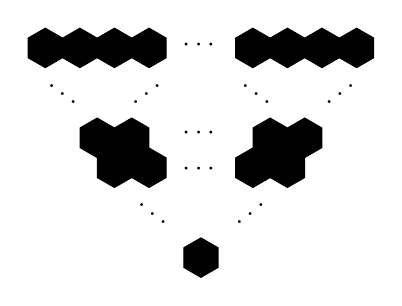
\begin{tikzpicture}[scale=0.25]
  %3^(k'+1)段目
  \filldraw[fill=\myRed,yshift={25*sqrt(3)*2}] (0,0)--++(30:1)--++(90:1)--++(150:1)--++(210:1)--++(270:1)--cycle;
  %3^k'+2 〜 3^(k'+1)-1段目
  \node[yshift={25*sqrt(3)*1.4}](0,0){$\cdots$};
  \node[xshift={-25*0.7},yshift={25*sqrt(3)*1.1}](0,0){$\ddots$};
  \node[xshift={25*0.7},yshift={25*sqrt(3)*1.1}](0,0){$\iddots$};
  %3^k'+1段目
  \filldraw[fill=\myRed,xshift={-25*5},yshift={25*sqrt(3)*5}] (0,0)--++(30:1)--++(90:1)--++(150:1)--++(210:1)--++(270:1)--cycle;
  \filldraw[fill=\myRed,xshift={-25*3},yshift={25*sqrt(3)*5}] (0,0)--++(30:1)--++(90:1)--++(150:1)--++(210:1)--++(270:1)--cycle;
  \node[yshift={25*sqrt(3)*1.7}](0,0){$\cdots$};
  \filldraw[fill=\myRed,xshift={25*3},yshift={25*sqrt(3)*5}] (0,0)--++(30:1)--++(90:1)--++(150:1)--++(210:1)--++(270:1)--cycle;
  \filldraw[fill=\myRed,xshift={25*5},yshift={25*sqrt(3)*5}] (0,0)--++(30:1)--++(90:1)--++(150:1)--++(210:1)--++(270:1)--cycle;
  %3^k'段目
  \filldraw[fill=\myYellow,xshift={-25*6},yshift={25*sqrt(3)*6}] (0,0)--++(30:1)--++(90:1)--++(150:1)--++(210:1)--++(270:1)--cycle;
  \filldraw[fill=\myBlue,xshift={-25*4},yshift={25*sqrt(3)*6}] (0,0)--++(30:1)--++(90:1)--++(150:1)--++(210:1)--++(270:1)--cycle;
  \filldraw[fill=\myBlue,xshift={25*4},yshift={25*sqrt(3)*6}] (0,0)--++(30:1)--++(90:1)--++(150:1)--++(210:1)--++(270:1)--cycle;
  \filldraw[fill=\myYellow,xshift={25*6},yshift={25*sqrt(3)*6}] (0,0)--++(30:1)--++(90:1)--++(150:1)--++(210:1)--++(270:1)--cycle;
  %1 〜 3^k'-1段目
  \node[xshift={-25*2},yshift={25*sqrt(3)*2.1}](0,0){$\ddots$};
  \node[xshift={-25*0.8},yshift={25*sqrt(3)*2.1}](0,0){$\iddots$};
  \node[xshift={25*0.8},yshift={25*sqrt(3)*2.1}](0,0){$\ddots$};
  \node[xshift={25*2},yshift={25*sqrt(3)*2.1}](0,0){$\iddots$};
  %0段目
  \filldraw[fill=\myYellow,xshift={-25*9},yshift={25*sqrt(3)*9}] (0,0)--++(30:1)--++(90:1)--++(150:1)--++(210:1)--++(270:1)--cycle;
  \filldraw[fill=\myBlue,xshift={-25*7},yshift={25*sqrt(3)*9}] (0,0)--++(30:1)--++(90:1)--++(150:1)--++(210:1)--++(270:1)--cycle;
  \filldraw[fill=\myYellow,xshift={-25*5},yshift={25*sqrt(3)*9}] (0,0)--++(30:1)--++(90:1)--++(150:1)--++(210:1)--++(270:1)--cycle;
  \filldraw[fill=\myBlue,xshift={-25*3},yshift={25*sqrt(3)*9}] (0,0)--++(30:1)--++(90:1)--++(150:1)--++(210:1)--++(270:1)--cycle;
  \node[yshift={25*sqrt(3)*2.3},above=0.01cm](0,0){$\cdots$};
  \filldraw[fill=\myBlue,xshift={25*3},yshift={25*sqrt(3)*9}] (0,0)--++(30:1)--++(90:1)--++(150:1)--++(210:1)--++(270:1)--cycle;
  \filldraw[fill=\myYellow,xshift={25*5},yshift={25*sqrt(3)*9}] (0,0)--++(30:1)--++(90:1)--++(150:1)--++(210:1)--++(270:1)--cycle;
  \filldraw[fill=\myBlue,xshift={25*7},yshift={25*sqrt(3)*9}] (0,0)--++(30:1)--++(90:1)--++(150:1)--++(210:1)--++(270:1)--cycle;
  \filldraw[fill=\myYellow,xshift={25*9},yshift={25*sqrt(3)*9}] (0,0)--++(30:1)--++(90:1)--++(150:1)--++(210:1)--++(270:1)--cycle;
\end{tikzpicture}

      \caption{$n$が奇数 かつ $3^{k} < n \leq 2 \cdot 3^{k}$}
      \label{fig:shortodd_steps}
    \end{figure}
  \item
    \ref{case:longodd}.のときは最上段のマスを両端のマスからそれぞれ$3^k$マス内側の方に向かって黄,その他の内側のマスを青を用いて対称的に塗る(図~\ref{fig:longodd_steps}参照).
    このとき,黄で塗られている内側のマスは$n-2\cdot3^k+1$マスである.
    %% ---------- 未修正 ----------
    すると,補題\ref{lem:tri_suf}より$3^k$段の逆三角形は調和彩色三角形なので,最上段から$3^k$段において外側から$n-2\cdot3^k+1$マスはすべて赤で塗られている.
    同様にして,$2\cdot3^k$段下のマスの色はすべて赤で塗られている.
    したがって,最上段の両端のマスの色は黄であり,最下段のマスの色が赤であるから調和性を満たさないので調和彩色三角形でない.
    %% ------------------------------
    \begin{figure}[h]
      \centering
      % oddshort_steps
\definecolor{grayR}{rgb}{0.50, 0.50, 0.50}
\definecolor{grayB}{rgb}{0.10, 0.10, 0.10}
\definecolor{grayY}{rgb}{1.00, 1.00, 1.00}
%\def\myRed{red}
%\def\myBlue{blue}
%\def\myYellow{yellow}
\def\myRed{grayR}
\def\myBlue{grayB}
\def\myYellow{grayY}

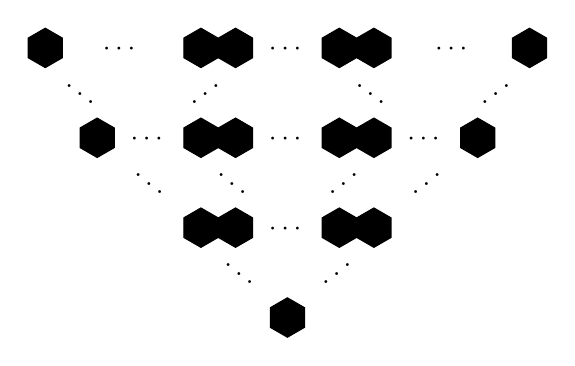
\begin{tikzpicture}[scale=0.25]
  %3^(k'+1)段目
  \filldraw[fill=\myRed,yshift={25*sqrt(3)*5}] (0,0)--++(30:1)--++(90:1)--++(150:1)--++(210:1)--++(270:1)--cycle;
  %3^k'+2 〜 3^(k'+1)-1段目
  \node[xshift={-25*0.7},yshift={25*sqrt(3)*1.85}](0,0){$\ddots$};
  \node[xshift={25*0.7},yshift={25*sqrt(3)*1.85}](0,0){$\iddots$};
  %3^k'+1段目
  \filldraw[fill=\myRed,xshift={-25*5},yshift={25*sqrt(3)*8}] (0,0)--++(30:1)--++(90:1)--++(150:1)--++(210:1)--++(270:1)--cycle;
  \filldraw[fill=\myRed,xshift={-25*3},yshift={25*sqrt(3)*8}] (0,0)--++(30:1)--++(90:1)--++(150:1)--++(210:1)--++(270:1)--cycle;
  \node[yshift={25*sqrt(3)*2.15}](0,0){$\cdots$};
  \filldraw[fill=\myRed,xshift={25*3},yshift={25*sqrt(3)*8}] (0,0)--++(30:1)--++(90:1)--++(150:1)--++(210:1)--++(270:1)--cycle;
  \filldraw[fill=\myRed,xshift={25*5},yshift={25*sqrt(3)*8}] (0,0)--++(30:1)--++(90:1)--++(150:1)--++(210:1)--++(270:1)--cycle;
  %3^k'+1 〜 3^(k'+1)-1段目
  \node[xshift={-25*2},yshift={25*sqrt(3)*2.6}](0,0){$\ddots$};
  \node[xshift={25*0.8},yshift={25*sqrt(3)*2.6}](0,0){$\iddots$};
  \node[xshift={-25*0.8},yshift={25*sqrt(3)*2.6}](0,0){$\ddots$};
  \node[xshift={25*2},yshift={25*sqrt(3)*2.6}](0,0){$\iddots$};
  %3^k'段目
  \filldraw[fill=\myRed,xshift={-25*11},yshift={25*sqrt(3)*11}] (0,0)--++(30:1)--++(90:1)--++(150:1)--++(210:1)--++(270:1)--cycle;
  \node[xshift={-25*2},yshift={25*sqrt(3)*2.9}](0,0){$\cdots$};
  \filldraw[fill=\myRed,xshift={-25*5},yshift={25*sqrt(3)*11}] (0,0)--++(30:1)--++(90:1)--++(150:1)--++(210:1)--++(270:1)--cycle;
  \filldraw[fill=\myYellow,xshift={-25*3},yshift={25*sqrt(3)*11}] (0,0)--++(30:1)--++(90:1)--++(150:1)--++(210:1)--++(270:1)--cycle;
  \node[yshift={25*sqrt(3)*2.9}](0,0){$\cdots$};
  \filldraw[fill=\myYellow,xshift={25*3},yshift={25*sqrt(3)*11}] (0,0)--++(30:1)--++(90:1)--++(150:1)--++(210:1)--++(270:1)--cycle;
  \filldraw[fill=\myRed,xshift={25*5},yshift={25*sqrt(3)*11}] (0,0)--++(30:1)--++(90:1)--++(150:1)--++(210:1)--++(270:1)--cycle;
  \node[xshift={25*2},yshift={25*sqrt(3)*2.9}](0,0){$\cdots$};
  \filldraw[fill=\myRed,xshift={25*11},yshift={25*sqrt(3)*11}] (0,0)--++(30:1)--++(90:1)--++(150:1)--++(210:1)--++(270:1)--cycle;
  %1 〜 3^k'-1段目
  \node[xshift={-25*3},yshift={25*sqrt(3)*3.35}](0,0){$\ddots$};
  \node[xshift={-25*1.2},yshift={25*sqrt(3)*3.35}](0,0){$\iddots$};
  \node[xshift={25*1.2},yshift={25*sqrt(3)*3.35}](0,0){$\ddots$};
  \node[xshift={25*3},yshift={25*sqrt(3)*3.35}](0,0){$\iddots$};
  %0段目
  \filldraw[fill=\myYellow,xshift={-25*14},yshift={25*sqrt(3)*14}] (0,0)--++(30:1)--++(90:1)--++(150:1)--++(210:1)--++(270:1)--cycle;
  \node[xshift={-25*2.4},yshift={25*sqrt(3)*3.65}](0,0){$\cdots$};
  \filldraw[fill=\myYellow,xshift={-25*5},yshift={25*sqrt(3)*14}] (0,0)--++(30:1)--++(90:1)--++(150:1)--++(210:1)--++(270:1)--cycle;
  \filldraw[fill=\myBlue,xshift={-25*3},yshift={25*sqrt(3)*14}] (0,0)--++(30:1)--++(90:1)--++(150:1)--++(210:1)--++(270:1)--cycle;
  \node[yshift={25*sqrt(3)*3.65}](0,0){$\cdots$};
  \filldraw[fill=\myBlue,xshift={25*3},yshift={25*sqrt(3)*14}] (0,0)--++(30:1)--++(90:1)--++(150:1)--++(210:1)--++(270:1)--cycle;
  \filldraw[fill=\myYellow,xshift={25*5},yshift={25*sqrt(3)*14}] (0,0)--++(30:1)--++(90:1)--++(150:1)--++(210:1)--++(270:1)--cycle;
  \node[xshift={25*2.4},yshift={25*sqrt(3)*3.65}](0,0){$\cdots$};
  \filldraw[fill=\myYellow,xshift={25*14},yshift={25*sqrt(3)*14}] (0,0)--++(30:1)--++(90:1)--++(150:1)--++(210:1)--++(270:1)--cycle;
\end{tikzpicture}

      \caption{$n$が奇数 かつ $2 \cdot 3^{k} + 1 \leq n < 3^{k+1}$}
      \label{fig:longodd_steps}
    \end{figure}
\end{itemize}


% 三角形三色問題の証明の Coq の実装の準備
\section{Coq 上で実装するための準備}
% 3.1 定義
% 関数 \mix・記号の説明
% WellColoredTriangle x y n c0 c1 c2 :=
% Cpos x y c0 /\ Cpos (x+n) y c1 /\ Cpos x (y+n) c2 -> c2 = \mix c0 c1
\subsection{調和彩色三角形の形式化}
本節では三角形三色問題の Coq 上での形式化の方法について,実装したコードの一部を挙げながら述べる
\footnote{紙面の都合上,実際とは異なる場所で改行されることがある.また,挙げているコードは可読性のため,{\tt forall} は$\forall$,{\tt exists} は$\exists$,{\tt nat} は$\mathbb{N}$,{\tt <=} は$\leq$で表示している.}.
使用する色の型 {\tt Color} の定義を以下で与える.
\begin{lstlisting}[language=Coq]
  Inductive Color : Set := red | yel | blu.
\end{lstlisting}

次に調和性を満たす3マスの色について,1つのマスの色は残りの2マスの色から決定される性質がある.
この性質を次の関数 {\tt mix} で表現する.
\begin{lstlisting}[language=Coq]
  Definition mix c0 c1 :=
  match c0, c1 with
  | red, red => red
  | red, yel => blu
  | red, blu => yel
  | yel, red => blu
  | yel, yel => yel
  | yel, blu => red
  | blu, red => yel
  | blu, yel => red
  | blu, blu => blu
  end.
\end{lstlisting}

前節での必要条件の証明 (定理~\ref{thm:tri_suf}) では,
{\tt mix}に関する性質を用いることで主張を示していた.
この性質は次の補題として記述される:
\begin{lstlisting}[language=Coq]
  Lemma mixcut c0 c1 c2 c3:
  mix (mix (mix c0 c1) (mix c1 c2)) (mix (mix c1 c2) (mix c2 c3)) = mix c0 c3.
Proof. by move: c0 c1 c2 c3 => [] [] [] []. Qed.
\end{lstlisting}
前節の脚注で述べた通り,この補題は (それぞれの場合は自明なものの) 81通りの場合分けを考慮する必要があるが,
最後のたった1行の記述で Coq は全ての場合分けの処理を完了している.

一般論として,幾何的な状況に関する問題はいくつかの暗黙の仮定が置かれていることが多い.
このような問題を形式化するには,暗黙の仮定を洗い出して観察し,適切な形式化の方法を選択する必要がある.
今回は「各場所には必ず1色のみが塗られること」が仮定されている.
そのため,彩色三角形全体の色塗りはマスの位置からそのマスの色を返す{\bf 彩色関数}として形式化する.
\begin{lstlisting}[language=Coq]
  Definition coloring := nat -> nat -> Color.
  Definition next cpos := forall x y,
       cpos x y.+1 = mix (cpos x y) (cpos x.+1 y).
\end{lstlisting}
上記の {\tt coloring} は彩色関数の型である.
以下,{\tt cpos} は彩色関数とし,{\tt cpos x y} は「左から{\tt x}段目,上から{\tt y}段目の色」を意味する.
また,{\tt next cpos}は「隣接するどの3つのマスも{\tt cpos}によって調和性を満たすように塗られている」を意味する.

次に彩色三角形の性質の定義を以下で与える:
\begin{lstlisting}[language=Coq]
  Definition Triangle cpos x y n :=
    cpos x (y + n) = mix (cpos x y) (cpos (x + n) y).
\end{lstlisting}
この {\tt Triangle cpos x y n} は


\begin{lstlisting}[language=Coq]
  Definition WellColoredTriangle x n := forall cpos,
    next cpos -> Triangle cpos x 0 n.
\end{lstlisting}

\begin{lstlisting}[language=Coq]
  Fixpoint liftcoloring (topcoloring : nat -> Color) x y :=
    if y is y'.+1 then mix (liftcoloring topcoloring x y') (liftcoloring topcoloring x.+1 y') else topcoloring x.
\end{lstlisting}


また,この問題では最上段の色を指定すれば色塗り規則に従えばその下の色も帰納的に求められるので,最上段の色塗りを与える関数から全体の色塗りを与える関数へ拡張できる.これらの観察結果が今回のCoq上での形式化のアイデアである.

まず,実装する際に用いた定義や関数,論理式について述べる.
以下,$f:A\to B\to C$のような型をもつ項と$a:A$と$b:B$について説明のために$f(a,b)$と記述することがあるが,
これは$f a b$と同義である.
\begin{dfn}[$\Color$]\rm
  マスに塗る色の集合を次のように定義する.
  \[
  \Color \eqDef \{\red, \yel, \blu\}.
  \]
  このとき,$\red$は{\rm{red}},$\yel$は{\rm{yellow}},$\blu$は{\rm{blue}}を表している.
  %% 以降,$\red$を$r$,$\yel$は$y$,$\blu$は$b$として略記することもある.
\end{dfn}
\begin{dfn}[$\mix$]\rm
  $\mix$ $:$ $\Color \to \Color \to \Color$ を以下で定義する.
  \[
  \begin{tabular}{cc}
    $(\red,\red) \Pto \red,$ & $(\red,\yel) \Pto \blu,$ \\
    $(\red,\blu) \Pto \yel,$ & $(\yel,\red) \Pto \blu,$ \\
    $(\yel,\yel) \Pto \yel,$ & $(\yel,\blu) \Pto \red,$ \\
    $(\blu,\red) \Pto \yel,$ & $(\blu,\yel) \Pto \red,$ \\
    $(\blu,\blu) \Pto \blu.$ \\
  \end{tabular}
  \]
\end{dfn}
演算 $\mix$ は塗り方の規則を再現するための関数の$1$つである.
引数となる$2$色が同じ場合は同じ色を返し,異なる場合は$2$色とも異なる第三の色を返す関数である.
\begin{dfn}[彩色関数]\rm
  マスの場所からそのマスの色を返す型$\N \to \N \to \Color$の関数を{\em 彩色関数}と呼ぶ.
  本稿では$\cpos$を彩色関数を意味する変数として用いることにし,$\cpos$の型を明記せずに省略することもある.
  $\cpos(x,y)$は左から $x$ 番目,上から $y$ 段目のマスの色を意味する.
\end{dfn}
\begin{exm}
  図$\ref{fig:nine_steps}$を与える色関数$\cpos$は,逆三角形の$3$つの端点のマスに関して
  次を満たす:
  \begin{itemize}
    \item $\cpos(0,0) = \yel,$
    \item $\cpos(9,0) = \blu,$
    \item $\cpos(0,9) = \red.$
  \end{itemize}
\end{exm}
\begin{dfn}[$\next$]\rm
  $\cpos : \N \to \N \to \Color$ に対して,
  $\next(\cpos)$を次のように定義する.

  $\next(\cpos)$ $\iffDef$
  $\forall$ $x,y \in\N,$
  $(\cpos(x,y+1)$ $=$ $\mix$ $(\cpos(x,y),$ $\cpos(x+1,y)).$
\end{dfn}
$\next$は互いに隣接する任意の$3$つのマスは調和性を満たしていることを論理式に書き直したものである.
すなわち,逆三角形に塗られている色はランダムに塗られているわけではなく,
$x,y$ を任意にすることで規則に従ってマスの色が塗られた彩色三角形で
あることを表している.

\begin{dfn}[$\WCT$]\rm
  $x, n \in \N$ に対して,
  $\WCT(x, n)$を次のように定義する:
  
  $\WCT(x, n)$ $\iffDef$ $(\forall \cpos: \N \to \N \to \Color, (\next(\cpos) \to \T(\cpos,x,0,n))$. \\
  ただし,$\T(\cpos,x,y,n)$ は以下で定義されている.

  $\T(\cpos,x,y,n) \iffDef
  \cpos(x,y+n) = \mix(cpos(x,y),cpos(x+n,y))$.
\end{dfn}
$\WCT$は定義$\ref{dfn:wc_tri}$で述べた$n$段の調和彩色三角形の定義を最上段の色の塗り方の関数$\cpos$を用いて論理式に書き直したものである.
$x$は逆三角形の左端のマス$(x,0)$
\footnote
    {
      左から$x$番目,上から$y$段目のマスを座標のように $(x,y)$ と表している.
      すなわち,$(x,0)$は左から$x$番目,上から$0$段目 (最上段) のマスを表している.
    }
    を基準として定めるために用いており,$n$は逆三角形の一辺の長さを表している.
    よって,三角形三色問題におけるマスの塗り方に従っていれば,彩色三角形の端点の$3$つのマス$(x,0), (x+n,0), (x,n)$に塗られている色は調和性を満たしていることを表している.

% 3.2 証明のための準備
\subsection{彩色条件} \label{sec:paint}
ここからはマスに塗る色の塗り方を表す関数について述べていく.
まず,最初に必要条件で用いる最上段のマスの塗り方を$3$つ紹介する.
\begin{dfn}[$\coloringYB$]\rm
  $\coloringYB$ $:$ $\N \to \N$ $\to$ $\Color$ を以下で定義する.

  $\coloringYB (n,x) \eqDef$
  \[
  \begin{cases}
    \yel & (x \leq n \land x\text{が奇数}) \\
    \blu & (\text{otherwise})
  \end{cases}
  \]
\end{dfn}
$\coloringYB$は補題$\ref{lem:tri_nec}$の証明において
$n$が偶数のときの最上段のマスの塗り方を表した関数である.
左端のマスから偶数番目のときは$\yel$,奇数番目のときは$\blu$を塗る.
すなわち,$\coloringYB$は最上段のマスを黄色と青で交互に塗る塗り方である.
\begin{dfn}[$\coloringYBBY$]\rm
  $\coloringYBBY :$ $\N \to \N$ $\to$ $\Color$ を以下で定義する.

  $\coloringYBBY(n,x) \eqDef$
  \[
  \begin{cases}
    \yel & (0 \leq x \leq n/2 \land x\text{が偶数}) \\
    \yel & (n/2+1 \leq x \leq n \land x\text{が奇数}) \\
    \blu & (\text{otherwise})
  \end{cases}
  \]
  ただし,$n/2$は分数ではなく商を表している.
\end{dfn}
$\coloringYBBY$は補題$\ref{lem:tri_nec}$の証明において$n$が奇数 かつ $3^{k} < n \leq 2 \cdot 3^{k}$のときの最上段のマスの塗り方を表した関数である.
$x \leq n/2$の範囲では左端のマスから偶数番目のときは$\yel$,奇数番目のときは$\blu$を塗り,$n/2+1 \leq x \leq n$の範囲では偶奇によって塗る色が入れ替わる.
すなわち,$\coloringYBBY$は外側から内側に向かって対称的に最上段のマスを
黄色と青で交互に塗る塗り方である.
\begin{dfn}[$\coloringBYB$]\rm
  $\coloringBYB$ $:$ $\N \to \N \to \N$ $\to$ $\Color$ を以下で定義する.

  $\coloringBYB(n,k,x) \eqDef$
  \[
  \begin{cases}
    \yel & (3^k \leq x \leq n-3^k) \\
    \blu & (\text{otherwise})
  \end{cases}
  \]
\end{dfn}
  $\coloringBYB$は補題$\ref{lem:tri_nec}$の証明において$n$が奇数かつ$2 \cdot 3^{k'} + 1 \leq n < 3^{k'+1}$のときの最上段のマスの塗り方を表した関数である.
  $\coloringBYB$は左端のマスから右の$3^k$番目のマスから$n-3^k$番目のマスまでの色を黄色で塗り,その他を青で塗っている.
すなわち,両端から$3^k$マスを青で塗り,その間を黄色で塗る塗り方である.

ここまで,最上段の色の塗り方を関数で表すことができた.
次は最上段のマスの塗り方 (関数) を
全体の色を決める彩色関数に拡張する関数を定義する.
\begin{dfn}[$\lift$]\rm
  $\lift : (\N\to\Color) \to \N \to \N \to \Color$ を以下で再帰的関数として定義する.
  
  $\lift(\topcolor,x,y) \eqDef$
  \[
  \begin{cases}
    \topcolor(x)
    \hfill (y = 0 \text{のとき}) \\
    \mix(\lift(\topcolor,x,y'),\lift(\topcolor,x+1,y')) & \\
    \hfill (y = y'+1 \text{のとき})
  \end{cases}
  \]
\end{dfn}
演算 $\lift$ は最上段の色塗りを与える関数$\topcolor$から全体の色塗りを与える彩色関数へ拡張する.
$y=0$ のときは最上段のマスは最上段の色塗り関数 $\topcolor$ に従って塗っていることを表している.
また,$y=y'+1$の形をしているときは,最上段から$y'$段目にある隣り合う$2$マスの色に対して,$\mix$を適用することでその間にある$y$段目のマスの色が得られることを表している.

% 3.3 補題
% mixcut, AllRed, rule
\subsection{関数の性質} \label{sec:lem}
次に証明を円滑に進めていくために用いた関数の性質に関する補題について述べる.
\begin{lem}[$\mixcut$] \label{lem:mixcut}
  $\forall c_0, c_1, c_2, c_3 \in \Color$に対して,
  $\mix( \mix ( \mix(c_0,c_1) , \mix(c_1,c_2) ), \mix( \mix(c_1,c_2),$ $\mix(c_2,c_3) ) ) = \mix(c_0,c_3)$.
\end{lem}
$\mixcut$は演算$\mix$のもつ性質を論理式にしたものであり,$\mix$と$4$色を用いて表された色は$2$色のみを用いて書き換えることができることを表している.
証明する際には各色が$3$通りずつ取り得るので合計$3^4=81$通りの場合分けをおこなって$\mix$の計算をすれば証明することができる.
三角形三色問題の十分条件$(\text{補題}\ref{lem:tri_suf})$を証明する際に用いる補題である.

\begin{lem}[$\AllRed$] \label{lem:AllRed}
  $\forall \cpos : \N \to \N \to \Color$,$x, y, n\in \N$ に対して,
  $\next(cpos)$ $\Imp$
  $(\forall i. \in \N,$ $(0 \leq i \leq n$ $\Imp$ $\cpos(x+i,y) = \red))$ $\Imp$
  $\cpos(x,y+n) = \red$.
\end{lem}
三角形三色問題の必要条件$(\text{補題}\ref{lem:tri_nec})$の証明において,$n$がどの場合でもすべてのマスが赤に塗られている段があることに帰着させて矛盾を導いている.
AllRedにより,すべてのマスが赤で塗られている段があるときは最下段のマスは赤であることがいえる.

\begin{lem}[$\cposF$] \label{lem:paint}
  $\forall \topcolor : \N \to \Color$ に対して,
  $\next(\lift(\topcolor)).$
\end{lem}
$\cposF$は$\lift(\topcolor)$に従ってマスの色を塗ると,常に$\next$を満たすことを表している.
すなわち,最上段のマスの塗り方を表す関数$\topcolor$が何であっても
これを拡張した彩色関数$\lift(\topcolor)$は互いに隣接する任意の$3$マスは調和性を
満たすこと表している.


% 三角形三色問題の概要(数学)
\section{Coqにおける三角形三色問題}

% 4.1 三角形三色問題の証明の Coq の実装(=>)
\subsection{十分条件}
補題\ref{lem:tri_suf}をCoqに実装するために論理式の形にしたものが次の定理\ref{thm:tri_suf}である.
\begin{thm}[十分条件] \label{thm:tri_suf}
  $\forall x, n \in \N, (\exists k \in \N, n = 3 ^ k \Imp \WCTF(x,n))$.
\end{thm}
\begin{proof}
  補題\ref{lem:tri_suf} (pp.\pageref{lem:tri_suf}) でも述べたように
  次を証明することで,定理\ref{thm:tri_suf}を示す.\\
  $\forall \cpos, \forall k, n, x, y \in \N,$ $n = 3^k \Imp (Fmix(\cpos) \Imp$ $\TF(cpos,x,y)).$ \\
  これを$k$に関する数学的帰納法を用いて証明する.
  $k=0$のときは$n=1$となるので明らかに成立する.
  次に$k$のとき成立すると仮定して$k+1$のときも成立することを示す.\\
  $3^k$マスずつ離れたマスの色を図\ref{fig:suf_steps}のように表すことにする.
  \begin{figure}[h]
    \centering
    % 3^{k'+1} 段の三角形
\begin{tikzpicture}
  {\normalsize{
      % 3^(k+1)段目
      \node (a0) {$c_{2}$};
      % 2*3^k段目
      \node[above left=0.5cm of a0] (b0) {$c_{8}$};
      \node[above right=0.5cm of a0] (b1) {$c_{9}$};
      % 3^k段目
      \node[above left=0.5cm of b0] (c0) {$c_{5}$};
      \node[above right=0.5cm of b0] (c1) {$c_{6}$};
      \node[above right=0.5cm of b1] (c2) {$c_{7}$};
      % 0段目
      \node[above left=0.5cm of c0] (d0) {$c_{0}$};
      \node[above right=0.5cm of c0] (d1) {$c_{3}$};
      \node[above left=0.5cm of c2] (d2) {$c_{4}$};
      \node[above right=0.5cm of c2] (d3) {$c_{1}$};
      % 点線 [3^(k+1)段 〜 2*3^k 段]
      \node[blue] at ($(a0)!.5!(b0)$) {$\ddots$};
      \node[blue] at ($(b0)!.5!(b1)$) {$\cdots$};
      \node[blue] at ($(a0)!.5!(b1)$) {$\iddots$};
      % 点線 [2*3^k 段 〜 3^k 段]
      \node[teal] at ($(b0)!.5!(c0)$) {$\ddots$};
      \node[teal] at ($(c0)!.5!(c1)$) {$\cdots$};
      \node[teal] at ($(b0)!.5!(c1)$) {$\iddots$};
      \node[red] at ($(b1)!.5!(c1)$) {$\ddots$};
      \node[red] at ($(c1)!.5!(c2)$) {$\cdots$};
      \node[red] at ($(b1)!.5!(c2)$) {$\iddots$};
      % 点線 [3^k 段 〜 0 段]
      \node[red] at ($(c0)!.5!(d0)$) {$\ddots$};
      \node[red] at ($(d0)!.5!(d1)$) {$\cdots$};
      \node[red] at ($(c0)!.5!(d1)$) {$\iddots$};
      \node[blue] at ($(c1)!.5!(d1)$) {$\ddots$};
      \node[blue] at ($(d1)!.5!(d2)$) {$\cdots$};
      \node[blue] at ($(c1)!.5!(d2)$) {$\iddots$};
      \node[teal] at ($(c2)!.5!(d2)$) {$\ddots$};
      \node[teal] at ($(d2)!.5!(d3)$) {$\cdots$};
      \node[teal] at ($(c2)!.5!(d3)$) {$\iddots$};
  }}
\end{tikzpicture}

    \caption{彩色三角形($n=3^{k+1}$のとき)}
    \label{fig:suf_steps}
  \end{figure}
  このとき,$3$つの端点のマスの色が$c_0=cpos(x,y^k)$,$c_3=cpos(x,y)$,
  $c_5=cpos(x+3^k,y^k)$である$3^k$段の彩色三角形が調和彩色三角形であることは,
  帰納法の仮定からすぐに示せる.
  同様にして,この彩色三角形以外にも$5$つの彩色三角形は調和彩色三角形である.
  すなわち,次の$6$つが成立する.
  \begin{itemize}
    \item $\TF(cpos,x,y,3^k)$
    \item $\TF(cpos,x+3^k,y,3^k)$
    \item $\TF(cpos,x+2\cdot3^k,y,3^k)$
    \item $\TF(cpos,x,y+3^k,3^k)$
    \item $\TF(cpos,x+3^k,y+3^k,3^k)$
    \item $\TF(cpos,x,y+2\cdot3^k,3^k)$
  \end{itemize}
  これらと補題\ref{lem:mixCut} $(\mixCut)$ を用いて式変形をすると,
  \[
  \cpos(x,y+3^k)=\mix(\cpos(x,y),\cpos(x+3^{k+1},y))
  \]
  が得られる.すなわち,$\TF(cpos,x,y,3^{k+1})$.\\
  したがって,$\TF(cpos,x,y,n)$である.
\end{proof}

% 4.2 三角形三色問題の証明の Coq の実装(<=)
% n が偶数の場合,n が奇数で短い場合,n が奇数で長い場合
% $n$が偶数のとき
% $n$が奇数 かつ $3^{k'} < n \leq 2 \cdot 3^{k}$のとき
% $n$が奇数 かつ $2 \cdot 3^{k'} + 1 \leq n < 3^{k+1}$のとき

\subsection{必要条件} \label{sec:nec}
補題\ref{lem:tri_nec}をCoqに実装するために論理式の形にしたものが次の定理\ref{thm:tri_nec}である.
\begin{thm}[必要条件] \label{thm:tri_nec}
  $\forall x, n \in \N, n > 0 \Imp$ \\
  $(\WCTF(x,n) \Imp \exists k \in , n = 3^k)$ 
\end{thm}
補題\ref{lem:tri_nec} (pp.\pageref{lem:tri_nec}) でも述べたように
次の対偶を証明することで定理\ref{thm:tri_nec}を示す.\\
$\forall n, x \in \N, n > 0 \Imp$
$(\lnot(\exists k \in \N, n = 3 ^ k) \Imp \lnot\WCTF(x,n))$ \\
この対偶を証明するためには,
\begin{itemize}
\item
  $n > 0$
\item
  $\lnot(\exists k \in \N, n = 3 ^ k)$,
\item
  $\WCTF(x,n)$
\end{itemize}
を仮定して矛盾を示せばよい.
今回は$n$に関する場合分けをしてから各場合において矛盾を導く.
\subsubsection{$n$が偶数}
$n$が偶数のときは補題\ref{lem:evenA},\ref{lem:evenB}を証明してから,補題\ref{lem:even}を証明して矛盾を導く.
\begin{lem}[\EvenA] \label{lem:evenA}
  $\forall \cpos, \forall x, n \in \N, n > 0  \Imp Fmix(\cpos) \Imp $
  $(\forall i \in \N, (0 \leq i \leq n \Imp \cpos(x+i,0) = \colorYB(x,n,x+i))) \Imp$
  $\forall i \in \N, (0 \leq i \leq n-1 \Imp \cpos(x+i,1) = red)).$
\end{lem}
補題\ref{lem:evenA}は最上段のマスの色を関数$\colorYB$で塗ると,最上段より$1$段下の段のマスの色はすべて赤であることを表している.
\begin{proof}
  $0$ $\leq$ $i$ $\leq$ $n-1$を満たす$i$を任意にとると,
  仮定より$\cpos(x+i,0) = \colorYB(x,n,x+i)$,$\cpos(x+i+1,0) = \colorYB(x,n,x+i+1)$.
  また,$\Fmix(\cpos)$より$\cpos(x+i,1) = \mix(\cpos(x+i,0),\cpos(x+i+1,0))$が導ける.
  \begin{itemize}
  \item
    $i$が偶数のとき \\
    $\colorYB$の定義より,$\colorYB(x,n,x+i)=\blu$,$\colorYB(x,n,x+i+1)=\yel$であるから$\cpos(x+i,1)=\red$.
  \item
    $i$が奇数のとき \\
    $\colorYB$の定義より,$\colorYB(x,n,x+i)=\yel$,$\colorYB(x,n,x+i+1)=\blu$であるから$\cpos(x+i,1)=\red$.
  \end{itemize}
  よって,$i$の遇奇にかかわらず$\cpos(x+i,1)=\red$.
\end{proof}
\begin{lem}[\EvenB] \label{lem:evenB}
  $\forall \cpos, \forall x, n \in \N, n > 0 \Imp \Fmix(\cpos) \Imp $
  $(\forall i \in \N, (0 \leq i \leq n \Imp \cpos(x+i,0) = \colorYB(x,n,x+i))) \Imp$
  $\cpos(x,n)=\red).$
\end{lem}
補題\ref{lem:evenB}は最上段のマスの色を関数$\colorYB$で塗ると,最下段のマスの色は赤になるということを表している.
\begin{proof}
  補題\ref{lem:evenA}より$\forall i \in \N, (0 \leq i \leq n-1 \Imp \cpos(x+i,1) = red)$.
  さらに,補題\ref{lem:AllRed}より$\cpos(x,n)=\red$.
\end{proof}

\begin{lem}[\Even] \label{lem:even}
  $\forall x,n \in \N,$ 
  $(n > 0 \land odd(n) = false) \Imp$ 
  $\lnot\WCTF(x,n)$.

ただし,補題\ref{lem:even}の中にある$odd(n)$は次のようにSSReflectで定義されている関数である.

自然数$n$に対して,
\[
odd(n) \eqDef
\begin{cases}
  true & \text{($n$が奇数)} \\
  false & (otherwise)
\end{cases}
\]
\end{lem}
\begin{proof}
  補題\ref{lem:paint}より
  $\exists \cposYB, \Fmix(\cposYB) \land \forall x_1, y_1 \in \N, \cposYB(x_1,y_1) = \lift(\colorYB(x,n),x_1,y_1)$.
  さらに,存在する $\cposYB$ をそのまま $\cposYB$ として名付けると,
  $\forall i \in \N, \colorYB(x,n,x+i) = \cposYB(x+i,0)$ を満たす.
  また,$0 \leq 0 \leq n$,$0 \leq n \leq n$を満たすので
  $\colorYB(x,n,x)=\colorYB(x,n,x+n)=\yel$.
  さらに,仮定より$\TF(\cpos,x,0,n)$であるから$\cposYB(x,n)=\yel$となる.
  一方で,補題\ref{lem:evenB}より$\cpos(x,n)=\red$となるので矛盾する.
\end{proof}

\subsubsection{$n$が奇数 かつ $3^{k} < n \leq 2 \cdot 3^{k}$}
$n$が奇数 かつ$3^{k'} < n \leq 2 \cdot 3^{k}$のときは補題\ref{lem:shortoddA},\ref{lem:shortoddB},\ref{lem:shortoddC}を証明してから,補題\ref{lem:shortodd}を証明して矛盾を導く.
\begin{lem}[\ShortOddA] \label{lem:shortoddA}
  $\forall \cpos, \forall x, n, k \in \N,$
  $(3^k < n \leq (3^k\cdot2) \land odd(n) = true) \Imp$
  $n > 0  \Imp Fmix(\cpos) \Imp $
  $(\forall x_1, y_1 \in \N, \TF(\cpos,x_1,y_1,3^k)) \Imp$
  $(\forall i \in \N, (0 \leq i \leq n \Imp \cpos(x+i,0) = \colorYBBY(x,n,x+i))) \Imp$
  $(\forall i \in \N, (0 \leq i \leq n - 3^k \Imp \cpos(x+i,3^k) = \colorYB(x,n-3^k,x+i))).$
\end{lem}
補題\ref{lem:shortoddA}は最上段のマスの色を関数$\colorYBBY$で塗ると,最上段より$3^k$下の段のマスは黄,青で交互に塗ってあることを表している.
\begin{proof}
  $0$ $\leq$ $i$ $\leq$ $n-3^k$を満たす$i$を任意にとると,
  $0 \leq i \leq n$,$0 \leq i+3^k \leq n$であるから仮定より,
  $\cpos(x+i,0) = \colorYBBY(x,n,x+i)$,
  $\cpos(x+i+3^k,0) = \colorYBBY(x,n,x+i+3^k))$.
  また,仮定の$\TF(\cpos,x+i,0,3^k)$より
  $\cpos(x+i,3^k)=\mix(\cpos(x+i,n),\cpos(x+i+3^k,0))$が成立する.
  さらに,$n$は奇数であり$0 \leq i \leq n/2$,$n/2+1 \leq i+3^k \leq n$を満たすので$\colorYBBY$,$\colorYB$の色は$i$の遇奇によって定まる.
  \begin{itemize}
  \item
    $i$が偶数のとき \\
    $\colorYBBY$の定義より$\colorYBBY(x,n,x+i)=\yel$,$\colorYBBY(x,n,x+i+3^k)=\yel$であり,$\colorYB$の定義より$\colorYB(x,n-3^k,x+i)=\yel$.
    よって,$\cpos(x+i,3^k)=\mix(\yel,\yel)=\yel=\colorYB(x,n-3^k,x+i)$.
  \item
    $i$が奇数のとき \\
    $\colorYBBY$の定義より$\colorYB(x,n,x+i)=\blu$,$\colorYB(x,n,x+i+3^k)=\blu$であり,$\colorYB$の定義より$\colorYB(x,n-3^k,x+i)=blu$
    よって,$\cpos(x+i,3^k)=\mix(\blu,\blu)=\blu=\colorYB(x,n-3^k,x+i)$.
  \end{itemize}
  以上より,$i$の遇奇にかかわらず$\cpos(x+i,3^k) = \colorYB(x,n-3^k,x+i))$.
\end{proof}

\begin{lem}[\ShortOddB] \label{lem:shortoddB}
  $\forall \cpos, \forall x, n, k \in \N,$
  $(3^k < n \leq 3^k \cdot 2 \land odd(n) = true) \Imp$
  $n > 0  \Imp Fmix(\cpos) \Imp $
  $(\forall x_1, y_1 \in \N, \TF(\cpos,x_1,y_1,3^k)) \Imp$
  $(\forall i \in \N, (0 \leq i \leq n \Imp \cpos(x+i,0) = \colorYBBY(x,n,x+i))) \Imp$
  $(\forall i \in \N, (0 \leq i \leq n - 3^k-1 \Imp cpos(x+i,3^k+1)= \red)).$
\end{lem}
補題\ref{lem:shortoddB}は最上段のマスの色を関数$\colorYBBY$で塗ると,最上段から$3^k+1$下の段のマスはすべて赤であるということを表している.
\begin{proof}
  補題\ref{lem:shortoddA}より$\forall i \in \N, (0 \leq i \leq n - 3^k \Imp \cpos(x+i,3^k) = \colorYB(x,n-3^k,x+i))$となるので,
  $\cpos(x+i,3^k) = \colorYB(x,n-3^k,x+i)$,
  $\cpos(x+i+1,3^k) = \colorYB(x,n-3^k,x+i+1)$.
  $\Fmix(\cpos)$より$\cpos(x+i,3^k+1) = \mix(\cpos(x+i,3^k),\cpos(x+i+1,3^k))$.
  ここで,補題\ref{lem:shortoddA}と同様にして $i$ の偶奇で場合分けをする.
  \begin{itemize}
  \item
    $i$が偶数のとき \\
    $\colorYB$の定義より$\colorYB(x,n-3^k,x+i)=\yel$,$\colorYB(x,n-3^k,x+i+1)=\blu$.
    よって,$\cpos(x+i,3^k+1)=\mix(\cpos(x+i,3^k),\cpos(x+i+1,3^k))=\mix(\yel,\blu)=\red$.
  \item
    $i$が奇数のとき \\
    $\colorYB$の定義より$\colorYB(x,n-3^k,x+i)=\blu$,$\colorYB(x,n-3^k,x+i+1)=\yel$.
    よって,$\cpos(x+i,3^k+1)=\mix(\cpos(x+i,3^k),\cpos(x+i+1,3^k))=\mix(\blu,\yel)=\red$.
  \end{itemize}
  以上より,$i$の遇奇にかかわらず$\cpos(x+i,3^k+1) = \red$.
\end{proof}

\begin{lem}[\ShortOddC] \label{lem:shortoddC}
  $\forall \cpos, \forall x, n, k \in \N,$
  $(3^k < n \leq 3^k \cdot 2 \land odd(n) = true) \Imp$
  $n > 0  \Imp Fmix(\cpos) \Imp $
  $(\forall x_1, y_1 \in \N, \TF(\cpos,x_1,y_1,3^k)) \Imp$
  $(\forall i \in \N, (0 \leq i \leq n \Imp \cpos(x+i,0) = \colorYBBY(x,n,x+i))) \Imp$
  $(\forall i \in \N, (0 \leq i \leq n - 3^k-1 \Imp \cpos(x,n)= \red)).$
\end{lem}
補題\ref{lem:shortoddC}は最上段のマスの色を関数$\colorYBBY$で塗ると,最下段のマスの色は赤になるということを表している.
\begin{proof}
  補題\ref{lem:shortoddB}より$\forall i \in \N, (0 \leq i \leq n - 3^k-1 \Imp cpos(x+i,3^k+1)= \red)$.
  さらに,補題\ref{lem:AllRed}より$\cpos(x,n)=\red$.
\end{proof}

\begin{lem}[\ShortOdd] \label{lem:shortodd}
  $\forall x, n, k \in \N,$
  $(3^k < n \leq 3^k \cdot 2 \land odd(n) = true) \Imp \lnot\WCTF(x,n).$
\end{lem}
\begin{proof}
  補題\ref{lem:paint}より
  $\exists \cposYBBY, \Fmix(\cposYBBY) \land \forall x_1, y_1 \in \N, \cposYBBY(x_1,y_1) = \lift(\colorYBBY$ $(x,n),x_1,y_1)$.
  さらに,存在する $\cposYBBY$ をそのまま $\cposYBBY$ として名付けると,
  $\forall i \in \N, \colorYBBY(x,n,x+i) = \cposYBBY(x+i,0)$ を満たす.
  これより$\colorYBBY(x,n,x) = \cposYBBY(x,0)$,$\colorYBBY(x,n,x+n) = $
  $\cposYBBY(x+n,0)$.
  $n$が奇数であるから$\colorYBBY(x,n,x)=\colorYBBY(x,n,x+n)$が成立するので,
  $\colorYBBY$ $(x,n,x)=\colorYBBY(x,n,x+n)=\yel$.
  さらに,仮定より$\TF(\cposYBBY,x,0,n)$であるから$\cposYBBY(x,n)=\yel$となる.
  一方で,定理\ref{thm:tri_suf},補題\ref{lem:shortoddC}より$\cpos(x,n)=\red$となるので矛盾する.
\end{proof}


\subsubsection{$n$が奇数 かつ $2 \cdot 3^{k} + 1 \leq n < 3^{k+1}$}
$n$が奇数 かつ$2 \cdot 3^{k} + 1 \leq n < 3^{k+1}$のときは補題\ref{lem:longoddA},\ref{lem:longoddB},\ref{lem:longoddC}を証明してから,補題\ref{lem:longodd}を証明して矛盾を導く.
\begin{lem}[\LongOddA] \label{lem:longoddA}
  $\forall \cpos, \forall x, n, k \in \N,$
  $(3^k \cdot 2 + 1 \leq n < 3^{k+1}) \Imp$
  $Fmix(\cpos) \Imp $
  $(\forall x_1, y_1 \in \N, \TF(\cpos,x_1,y_1,3^k)) \Imp$
  $(\forall i \in \N, (0 \leq i \leq n \Imp \cpos(x+i,0) = \colorBYB(x,n,x+i))) \Imp$
  $($
   $(\forall i \in \N,(0 \leq i \leq n - 3^k \cdot 2 \Imp \cpos(x+i,3^k) = \red))$
   $\land$
   $(\forall i \in \N,(3^k \leq i \leq n - 3^k \Imp \cpos(x+i,3^k)=\red))$
  $)$.
\end{lem}
補題\ref{lem:longoddA}は最上段のマスの色を関数$\colorBYB$で塗ると,最上段より$3^k$下の段のマスは外側から$n-2\cdot3^k+1$マスはすべて赤で塗られていることを表している.
\begin{proof}
  $3^k\cdot2 + 1 \leq n < 3^{k+1}$を満たす$n$をとる.
  \begin{itemize}
  \item
    $\forall i \in \N,(0 \leq i \leq n - 3^k \cdot 2 \Imp \cpos(x+i,3^k) = \red)$を示す.\\
    $0$ $\leq$ $i$ $\leq$ $n - 3^k \cdot 2$を満たすように任意に$i$をとると,
    $0 \leq i \leq n$,$0 \leq i \leq 3^k-1$を満たすので,
    仮定より$\cpos(x+i,0)=\colorBYB(x,n,k,x+i)$であり,$\colorBYB(x,n,k,x+i)=\blu$が導ける.
    よって,$\cpos(x+i,0)=\blu$.
    また,$0 \leq i+3^k \leq n$,$3^k \leq i+3^k \leq n-3^k$を満たすので,
    $\cpos(x+i+3^k,0)=\colorBYB(x,n,k,x+i+3^k)$であり,$\colorBYB(x,n,k,x+i+3^k)=\yel$が導ける.
    よって,$\cpos(x+i+3^k,0)=\yel$.
    さらに,仮定より$\TF(\cpos,x+i,0,3^k)$だから$cpos(x+i,3^k)=\mix(\cpos(x+i,0)=\colorBYB(x,n,k,x+i),\cpos(x+i+3^k,0))=\mix(\blu,\yel)=\red$が成立する.
    よって,$\cpos(x+i,3^k)=\red$.
  \item
    $\forall i \in \N,(3^k \leq i \leq n - 3^k \Imp \cpos(x+i,3^k)=\red))$を示す.\\
    $3^k$ $\leq$ $i$ $\leq$ $n - 3^k$を満たすように任意に$i$をとると,
    $0 \leq i \leq n$,$3^k \leq i \leq n-3^k$を満たすので,
    仮定より$\cpos(x+i,0)=\colorBYB(x,n,k,x+i)$であり,$\colorBYB(x,n,k,x+i)=\yel$が導ける.
    よって,$\cpos(x+i,0)=\yel$.
    また,$0 \leq i+3^k \leq n$,$3^k \leq i+3^k \leq n-3^k$を満たすので,
    $\cpos(x+i+3^k,0)=\colorBYB(x,n,k,x+i+3^k)$であり,$\colorBYB(x,n,k,x+i+3^k)=\blu$が導ける.
    よって,$\cpos(x+i+3^k,0)=\blu$.
    さらに,仮定より$\TF(\cpos,x+i,0,3^k)$だから$cpos(x+i,3^k)=\mix(\cpos(x+i,0)=\colorBYB(x,n,k,x+i),\cpos(x+i+3^k,0))=\mix(\yel,\blu)=\red$が成立する.
    よって,$\cpos(x+i,3^k)=\red$.
  \end{itemize}
\end{proof}

\begin{lem}[\LongOddB] \label{lem:longoddB}
  $\forall \cpos, \forall x, n, k \in \N,$
  $(3^k \cdot 2 + 1 \leq n < 3^{k+1}) \Imp$
  $Fmix(\cpos) \Imp $
  $(\forall x_1, y_1 \in \N, \TF(\cpos,x_1,y_1,3^k)) \Imp$
  $(\forall i \in \N, (0 \leq i \leq n \Imp \cpos(x+i,0) = \colorBYB(x,n,x+i))) \Imp$
  $\forall i \in \N,$ $(0 \leq i \leq n - 3^k \cdot 2 \Imp \cpos(x+i,3^k \cdot 2) = red).$
\end{lem}
補題\ref{lem:longoddB}は最上段のマスの色を関数$\colorBYB$で塗ると,最上段から$3^k\cdot2$下の段のマスはすべて赤で塗られていることを表している.
\begin{proof}
  $0 \leq i \leq n - 3^k \cdot 2$を満たす$i$を任意にとると,
  補題\ref{lem:longoddA}より$\cpos(x+i,3^k) = red$.
  また,$3^k$ $\leq$ $i+3^k$ $\leq$ $n - 3^k$でもあるから
  補題\ref{lem:longoddA}より$\cpos(x+i+3^k,3^k) =\red$.
  さらに,仮定より$\TF(\cpos,x+i,3^k,3^k)$だから
  $cpos(x+i,3^k \cdot 2)=\mix(\cpos(x+i,3^k),\cpos(x+i+3^k,3^k))=\mix(\red,\red)=\red$.
  よって,$\cpos(x+i,3^k \cdot 2)=\red$.
\end{proof}

\begin{lem}[\LongOddC] \label{lem:longoddC}
  $\forall \cpos, \forall x, n, k \in \N,$
  $(3^k \cdot 2 + 1 \leq n < 3^{k+1}) \Imp$
  $Fmix(\cpos) \Imp $
  $(\forall x_1, y_1 \in \N, \TF(\cpos,x_1,y_1,3^k)) \Imp$
  $(\forall i \in \N, (0 \leq i \leq n \Imp \cpos(x+i,0) = \colorBYB(x,n,x+i))) \Imp$
  $\cpos(x,n) = \red$
\end{lem}
補題\ref{lem:longoddC}は最上段のマスの色を関数$\colorBYB$で塗ると,最下段のマスは赤になることを表している.
\begin{proof}
  補題\ref{lem:longoddB}より$\forall i \in \N,$ $(0 \leq i \leq n - 3^k \cdot 2 \Imp \cpos(x+i,3^k \cdot 2) = red).$
  さらに,補題\ref{lem:AllRed}より$\cpos(x,n)=\red$.
\end{proof}
\begin{lem}[\LongOdd] \label{lem:longodd}
  $\forall x, n, k \in \N,$
  $(3^k\cdot2 + 1 \leq n < 3^{k+1} \land odd(n) = true) \Imp \lnot\WCTF(x,n).$
\end{lem}
\begin{proof}
  補題\ref{lem:paint}より
  $\exists \cposBYB, \Fmix(\cposBYB) \land \forall x_1, y_1 \in \N, \cposBYB(x_1,y_1) = \lift(\colorBYB$ $(x,n),x_1,y_1)$.
  さらに,存在する $\cposBYB$ をそのまま $\cposBYB$ として名付けると,
  $\forall i \in \N, \cposBYB(x+i,0) = colorBYB(x,n,k,x+i)$ を満たす.
  これより$\cposBYB(x,0) = \colorBYB(x,n,k,x)$,$\cposBYB(x+n,0) = $
  $\colorBYB$ $(x,n,k,x+n)$.
  また,$0 \leq 0 \leq 3^k-1$,$n-3^k+1 \leq n \leq n$より
  $\colorBYB(x,n,k,x)=\colorBYB(x,n,k,x+n)=\blu$.
  さらに,仮定より$\TF(\cposBYB,x,0,n)$であるから
  $\cposYBBY(x,n)=\mix(\cposBYB(x,0),\cposBYB(x+n,0))=\mix(\blu,\blu)=\blu$
  となる.
  一方で,定理\ref{thm:tri_suf},補題\ref{lem:longoddC}より
  $\cpos(x,n)=\red$となるので矛盾する.
\end{proof}

以上より補題\ref{lem:even},\ref{lem:shortodd},\ref{lem:longodd}から
\ref{sec:nec}節の冒頭で述べた定理\ref{thm:tri_nec}を証明された.
さらに,定理\ref{thm:tri_suf}(十分条件),定理\ref{thm:tri_nec}(必要条件)が
成立するので定理\ref{thm:tri_iff}(必要十分条件)も示された.

\section{形式化するにあたって}
今回,Coq + SSReflect を用いて三角形三色問題の証明の形式化を完成させることができた.ここでは,形式化を完成させるにあたって経験したことや得られた知見について述べる.

$1$つ目として挙げるのは,形式化をする際には,形式化する方針をしっかりと考え,計画を立ててから実装するべきである.なぜなら,形式化の方針によっては Coq で実装するコードの行数を抑えられるからである.実際,$2021$ 年 $9$ 月に公開していたコードは約 $1200$ 行であったが,形式化の方針を変えて新しく $2021$ 年 $10$ 月で公開した三角形三色問題のコード
\footnote{
  \ref{sec:start}章でも述べたが,
  \url{https://github.com/SyotaHashimoto/ThreeColor} から
  完成させたCoqのコード (``Coqによる三角形三色問題の証明.v'') を
  ダウンロードすることができる.
}
は約 $900$ 行となり約 $300$ 行も減らすことができた.$9$ 月に公開していたコードでの実装では,述語を用いた命題や主張で実装をしていた.例えば,左から $x$ 番目,上から $y$ 番目のマスに塗られている色は $c$ であることを述語 $Cpos(x,y,c)$ とし,この述語が表す内容を公理を用いて定めることで命題や主張を表していた.一方で,新しく $10$ 月に公開したコードでは述語 $Cpos(x,y,c)$ ではなく,$\cpos$ や $\lift$ といった関数を用いて書き直すことができた.また,今回のように述語ではなく関数を用いて形式化すると,実装するコードの行数を大幅に削減できるだけでなく,公理を用意する必要がなくなるというメリットもあることもわかった.これは公理でマスに塗られる色は$1$色のみ存在することを保証していたが,関数に書き直すことで一意性を常に満たすからである.

$2$つ目としては,SSReflect を用いる際にはできる限り bool 型で実装することである.SSReflect には命題や主張をブール型と見なすことで証明を支援する機能が備わっている.そのため,SSReflect を用いる際には Prop 型ではなく bool 型として実装することで,様々な SSReflect の恩恵をうけることができる.例えば,bool 型で書かれた命題や主張はタクティック rewrite を用いることで真理値を計算したり,変形することで容易に証明することができる.
また,関数を定義する際に if 文を用いることがあるが,if 文の条件部分は bool 型を要求する.こういった側面からも Prop 型ではなく bool 型で実装した方が良いと考えられる.

一方で,$\forall$,$\exists$ が入った論理式は bool 型になおすことが困難であるため,今回の形式化を完成させる際に用いた $\Fmix$ は bool 型になおすことができなかった.したがって,$\WCTF$ は $\Fmix$ を含むので bool 型になおすことができず,形式化するにあたって用いたすべての主張や命題を bool 型を書き直すことができなかった.もし,この問題が解決することができたときには,更に形式化を完成させるためのコードを減らすことができるのではないかと考えられる.



%% 目標:これで得られた知見をまとめる (読者との情報共有)
%% - 形式化の最初の方針が肝心.上手い選択をすると証明の行数が大幅に削減できる
%% - 述語はやめる.関数で書けるならそっちの方がよい.
%% --- 自然と rewrite を使うことになるので ssreflect の利点を生かすことになる.
%% - できることなら Prop でなく bool で統一した方が ssreflect の利点が生きる
%% --- 関数定義をする際に if 文を用いると条件は bool 型を要求されるため,
%% --- 条件部分の述語は Prop 型でなく bool 型で最初から定義するとよい
%% -- forall や exists が入った論理式は無理そう
%% -- この理由により F_mix は bool にはできなかった
%% -- WellColoredTriangleF は F_mix を含むので bool にできなかった
%% - 紙に証明を書いてから実装するべし
%% -- 証明の設計は大事.全体の方針が見えるように上手く補題を立てるべし

% 結論,まとめ
\section{まとめ}
本研究では $\cpos$ や $\lift$ といった関数等を適切に定めることで
三角形三色問題の幾何的な状況を再現しつつ,
三角形三色問題の証明の形式化を Coq + SSReflect を用いて完成させることができた.

%       Bibliography 

\begin{thebibliography}{99}

\bibitem{Coq}
  ``The Coq Proof Assistant'',
  https://coq.inria.fr/. 

\bibitem{SSReflect}
  ``The SSReflect proof language'',
  \\
  https://coq.inria.fr/refman/proof-engine/ssreflect-proof-language.html. 
  
\bibitem{CoqBook}
  萩原学, アフェルド・レナルド, 
  ``Coq/SSReflect/MathComp による定理証明'',
  森北出版,
  2018. 
  
\bibitem{Nishiyama1}
  西山豊,
  ``エレガントな解答をもとむ 出題2'',
  数学セミナー,
  4月号, pp.87--91, 2013.
  
\bibitem{Nishiyama2}
  西山豊,
  ``数学を楽しむ/三角形三色問題'',
  現代数学,
  Vol.47, No.10, pp.36--41, 2014.
  
\bibitem{Nishiyama3}
  Y.~Nishiyama,
  ``THE THREE-COLOR TRIANGLE PROBLEM'', 
  International Journal of Pure and Applied Mathematics,
  Vol.85, No.1, pp.69--81, 2013.

\end{thebibliography}

%\input{authors}

\end{document}
